\subsection{Exercise 1}
We consider a single parent individual \(x_0\) (which is a vector of real value parameters) from which we create a number of offspring individuals according to a Gaussian perturbation (we add a random number from a Gaussian to each parameter \(x_i\)) of the parent
\begin{itemize}
    \item \textit{Do the mutations tend to improve or worsen the fitness of the parent?} Being the mutation based on a Gaussian with mean 0 this means there is an equal probability that the mutation improves or worsen the value for the parent in one of the dimensions. The improvement in the fitness of the individuals derives from running the algorithm for multiple generation and, for each generation, select the only the individuals with a good fitness value as the parents for the following generation
    \item \textit{Are low or high mutation magnitudes best for improving the fitness? How does this depend on the initial value of the parent and on the number of dimensions of the search space?}High mutation magnitudes perturb the parent more thus is desirable if the parent is far from the minimum of the fitness function while if the parent is close to the minimum a large mutation could lead to "missing" the minimum (similarly to how the learning rate in nn is larger at the beginning and then decreases)
\end{itemize}

%$f(\mathbf{x}) = \sum_{i=1}^{N}{x^2_i}$
\subsection{Exercise 2}
\subsubsection{Changes in size of parameter space}
\begin{lstlisting}
# Number of dimensions
num_vars_1 = 2;
num_vars_2 = 10;
num_vars_3 = 50;
# How close the parent is to the minimum
value_1 = 10;
value_2 = 10;
value_3 = 10;
# standard deviation of the mutation
std_dev_1 = 1;
std_dev_2 = 1;
std_dev_3 = 1;
\end{lstlisting}
\begin{figure}[H]
    \centering
    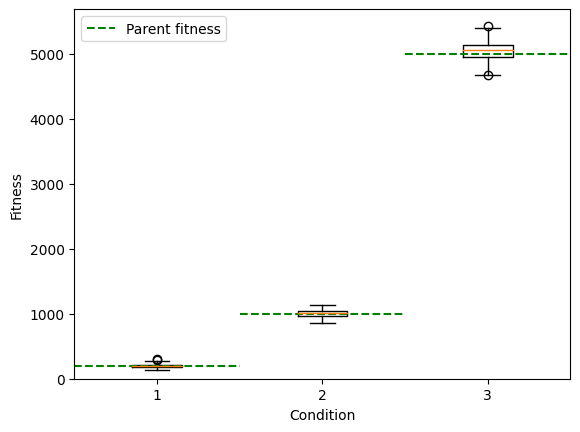
\includegraphics[width=\linewidth]{images/lab1/diff_dimensions.png}
    \caption{Larger number of dimensions lead to a worse fitness since each to each dimension we apply a Gaussian mutation independently from the other dimensions. These means that a larger number of mutations need to be favorable when we have more dimensions in order to have an overall positive effect on the fitness function}
    \label{fig:my_label}
\end{figure}
\begin{lstlisting}
mean for condition 1 199.0270683313231
mean for condition 2 1007.8578674815335
mean for condition 3 5052.458821293098
t test for condition 1 TtestResult(statistic=-0.48352189402190093, pvalue=0.6292568165960182, df=199)
t test for condition 2 TtestResult(statistic=1.8857158602849116, pvalue=0.060790116886670645, df=199)
t test for condition 3 TtestResult(statistic=5.16512983485652, pvalue=5.812656389863935e-07, df=199)   
\end{lstlisting}



\subsubsection{Changes in parent position}


\subsubsection{Changes in standard deviation}
\begin{lstlisting}
# Number of dimensions
num_vars_1 = 10;
num_vars_2 = 10;
num_vars_3 = 10;
# How close the parent is to the minimum
value_1 = 50;
value_2 = 50;
value_3 = 50;
# standard deviation of the mutation
std_dev_1 = 1;
std_dev_2 = 5;
std_dev_3 = 10;
\end{lstlisting}
\begin{figure}[H]
    \centering
    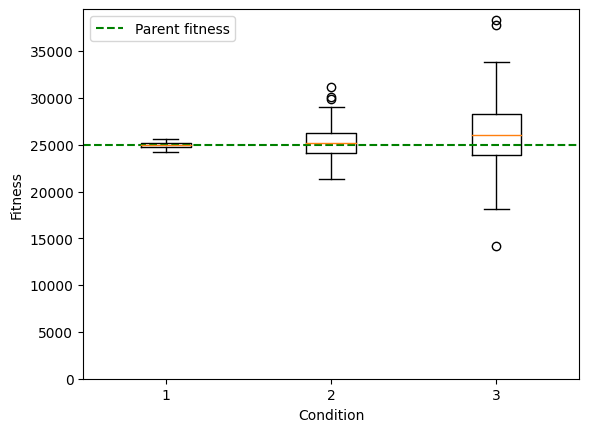
\includegraphics[width=\linewidth]{images/lab1/diff_var.png}
    \caption{Different standard deviations, we can see how larger standard deviations lead to bigger spreads of the fitness function of the offspring}
\end{figure}
\begin{lstlisting}
mean for condition 1 24992.395153622747
mean for condition 2 25273.758454594732
mean for condition 3 26136.27440484417
t test for condition 1 TtestResult(statistic=-0.3502566629937968, pvalue=0.7265165337240436, df=199)
t test for condition 2 TtestResult(statistic=2.428150584493876, pvalue=0.01606526209812561, df=199)
t test for condition 3 TtestResult(statistic=4.688702475083695, pvalue=5.097289331034417e-06, df=199)
\end{lstlisting}


\begin{lstlisting}
# Number of dimensions
num_vars_1 = 10;
num_vars_2 = 10;
num_vars_3 = 10;
# How close the parent is to the minimum
value_1 = 10;
value_2 = 10;
value_3 = 10;
# standard deviation of the mutation
std_dev_1 = 1;
std_dev_2 = 5;
std_dev_3 = 10;
\end{lstlisting}
\begin{figure}[H]
    \centering
    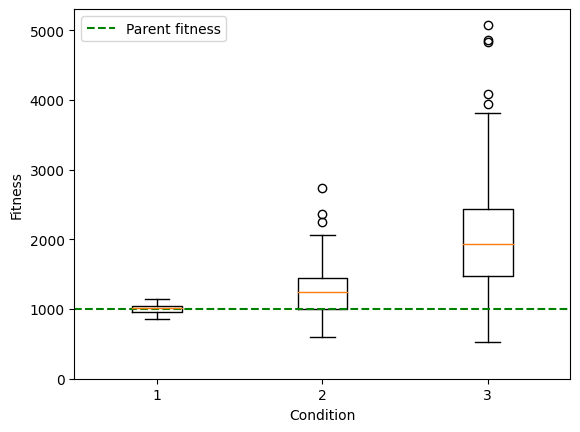
\includegraphics[width=\linewidth]{images/lab1/diff_var_close_to_optim.png}
    \caption{Different standard deviations; we can see how larger standard deviations for parents near the optimum lead to worst offspring fitness. In a one dimensional case we can think of this as "skipping" the minimum of the Gaussian with the perturbation and ending up on the other side.}
\end{figure}
\begin{lstlisting}
mean for condition 1 1006.6851110793099
mean for condition 2 1255.275188175959
mean for condition 3 2021.868806317667
t test for condition 1 TtestResult(statistic=1.5430590255274772, pvalue=0.12440515769783138, df=199)
t test for condition 2 TtestResult(statistic=10.617486211324527, pvalue=3.748620582911768e-21, df=199)
t test for condition 3 TtestResult(statistic=17.85706148017013, pvalue=3.3609390306894233e-43, df=199)
 
\end{lstlisting}

\subsection{Exercise 3}
\subsubsection{1D case}
\begin{figure}[H]
    \centering
    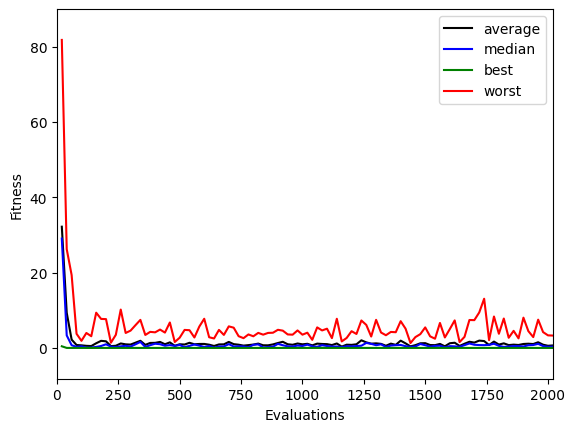
\includegraphics[width=\linewidth]{images/lab1/fitness_1D.png}
    \caption{1D case with initial conditions (sd=1, n\_generations=100)}
\end{figure}
\begin{lstlisting}
Best Individual: [-0.0007493]
Best Fitness: 5.614550796941787e-07
Distance from Global Optimum 0.0007493030626483377
\end{lstlisting}

\subsubsection{Multidimensional case (10D)}
\begin{figure}[H]
    \centering
    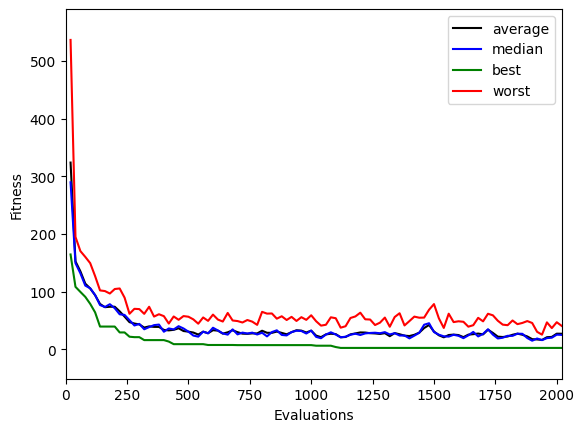
\includegraphics[width=\linewidth]{images/lab1/fitness_10D.png}
    \caption{1D case with initial conditions (sd=1, n\_generations=100). We can see how it's much harder to reach the minimum in higher dimensional spaces}
\end{figure}
\begin{lstlisting}
Best Individual: [ 0.30053474  0.02030438 -0.28887405 -0.64750114  0.1414396  -0.10231473 -0.94934182 -0.83373845  0.11002579  0.17005845]
Best Fitness: 2.26130806375365
Distance from Global Optimum 1.5037646304371073
\end{lstlisting}

\begin{figure}[H]
    \centering
    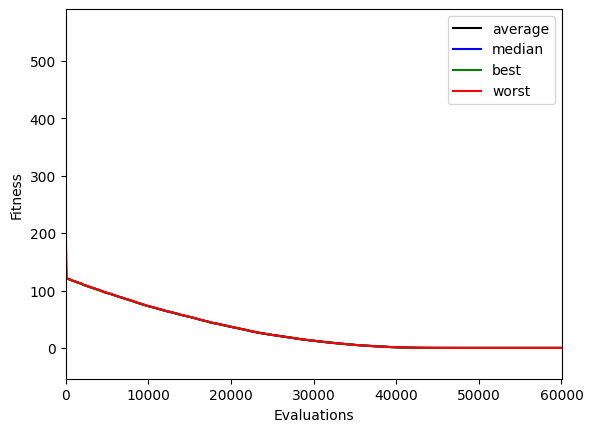
\includegraphics[width=\linewidth]{images/lab1/fitness_10D_better.png}
    \caption{sd=0.005 and 3000 generations}
\end{figure}
\begin{lstlisting}
Best Individual: [-0.00319792 -0.00083481 -0.0007718   0.00147632 -0.0003382   0.00382437 0.00231973  0.00418892  0.00013882  0.00027812]
Best Fitness: 5.146382897339173e-05
Distance from Global Optimum 0.007173829449700608
\end{lstlisting}
Using a small standard deviation we perturb an individual less than with a larger mutation, but given enough generations we can achieve a very good result (even if we're still a order of magnitude off from the 1D case.

\begin{figure}[H]
    \centering
    \begin{subfigure}[t]{0.5\textwidth}
        \centering
        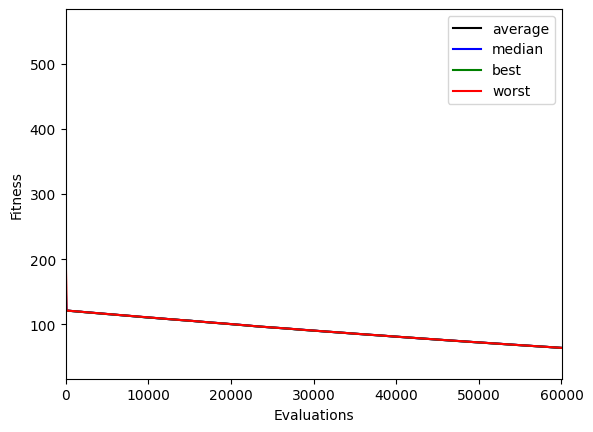
\includegraphics[width=\linewidth]{images/lab1/fitness_10D_small_sd.png}
        \captionsetup{format=hang}
        \caption{sd=0.001, too small, not enough \\perturbation to reach minimum \\(distance 7.997124392959498)}
    \end{subfigure}%
    \begin{subfigure}[t]{0.5\textwidth}
        \centering
        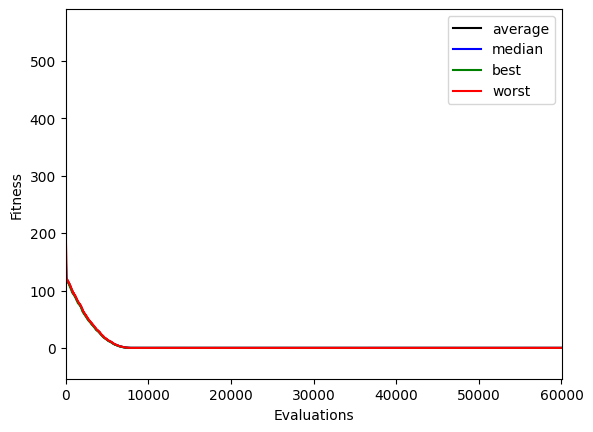
\includegraphics[width=\linewidth]{images/lab1/fitness_10D_big_sd.png}
        \captionsetup{format=hang}
        \caption{sd=0.03, too big, bounce around the minimum (distance 0.03196880703719635)}
    \end{subfigure}
\end{figure}

\subsection{Exercise 4}
\begin{figure}[H]
    \centering
    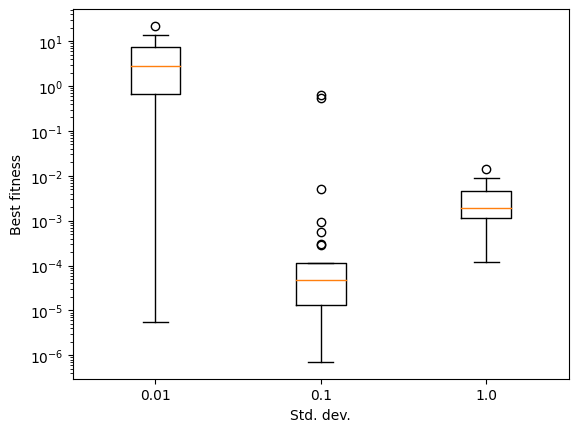
\includegraphics[width=\linewidth]{images/lab1/compare_fitness.png}
    \caption{standard conditions (n\_generations=50, 30 runs per standard deviation) }
\end{figure}

\begin{figure}[H]
    \centering
    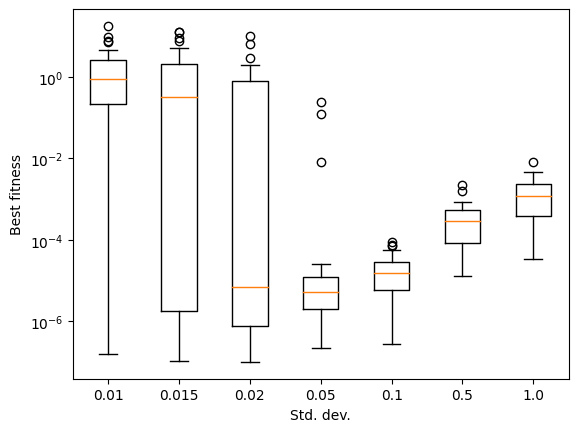
\includegraphics[width=\linewidth]{images/lab1/compare_fitness_1.png}
    \caption{We can see the different behaviours with more standard deviations (n\_generations=100)}
\end{figure}